\documentclass[a4paper,12pt]{article}

\usepackage{float}


\usepackage[utf8]{inputenc}
\usepackage[dvips]{graphicx}
%\usepackage{a4wide}
\usepackage{epsfig}
\usepackage{fancybox}
\usepackage{verbatim}
\usepackage{array}
\usepackage{latexsym}
\usepackage{alltt}
\usepackage{amssymb}
\usepackage{amsmath,amsthm}
\usepackage{bm}
\usepackage{wasysym}

%\usepackage{fullpage}
%\usepackage{hyperref}
\usepackage{listings}
\usepackage{color}
\usepackage{algorithm}
\usepackage{algpseudocode}
\usepackage[hmargin=2cm,vmargin=3.0cm]{geometry}
%\topmargin=0cm
%\topmargin=-1.8cm
%\addtolength{\textheight}{6.5cm}
%\addtolength{\textwidth}{2.0cm}
%\setlength{\leftmargin}{-3cm}
%\setlength{\oddsidemargin}{0.0cm}
%\setlength{\evensidemargin}{0.0cm}

%misc libraries goes here
\usepackage{tikz}
\usepackage{tikz-qtree}
\usetikzlibrary{automata,positioning}

\usepackage{multicol}
\usepackage{enumitem}

\usepackage[most]{tcolorbox}

\usepackage[colorlinks=true,urlcolor=black,linkcolor=black]{hyperref}


\lstdefinestyle{customtex}{
    %backgroundcolor=\color{lbcolor},
    tabsize=2,
    language=TeX,
    numbers=none,
    basicstyle=\footnotesize\ttfamily,
    numberstyle=\footnotesize,
    aboveskip={0.0\baselineskip},
    belowskip={0.0\baselineskip},
    %
    columns=flexible,
    keepspaces=true,
    fontadjust=true,
    upquote=true,
    %
    breaklines=true,
    prebreak=\raisebox{0ex}[0ex][0ex]{\ensuremath{\hookleftarrow}},
    frame=single,
    showtabs=false,
    showspaces=false,
    showstringspaces=false,
    %
    %identifierstyle=\color[rgb]{0,0.2,0.8},
    identifierstyle=\color[rgb]{0,0,0.5},
    %identifierstyle=\color[rgb]{0.133,0.545,0.133},
    %keywordstyle=\color[rgb]{0.8,0,0},
    %keywordstyle=\color[rgb]{0.133,0.545,0.133},
    keywordstyle=\color[rgb]{0,0,0.5},
    %commentstyle=\color[rgb]{0.133,0.545,0.133},
    commentstyle=\color[rgb]{0.545,0.545,0.545},
    %stringstyle=\color[rgb]{0.827,0.627,0.133},
    stringstyle=\color[rgb]{0.133,0.545,0.133},
    %
    literate={â}{{\^{a}}}1 {Â}{{\^{A}}}1 {ç}{{\c{c}}}1 {Ç}{{\c{C}}}1 {ğ}{{\u{g}}}1 {Ğ}{{\u{G}}}1 {ı}{{\i}}1 {İ}{{\.{I}}}1   {ö}{{\"o}}1 {Ö}{{\"O}}1 {ş}{{\c{s}}}1 {Ş}{{\c{S}}}1 {ü}{{\"u}}1 {Ü}{{\"U}}1 {~}{$\sim$}{1}
}

\lstdefinestyle{output}{
    %backgroundcolor=\color{lbcolor},
    tabsize=2,
    numbers=none,
    basicstyle=\footnotesize\ttfamily,
    numberstyle=\footnotesize,
    aboveskip={0.0\baselineskip},
    belowskip={0.0\baselineskip},
    %
    columns=flexible,
    keepspaces=true,
    fontadjust=true,
    upquote=true,
    %
    breaklines=true,
    prebreak=\raisebox{0ex}[0ex][0ex]{\ensuremath{\hookleftarrow}},
    frame=single,
    showtabs=false,
    showspaces=false,
    showstringspaces=false,
    %
    %identifierstyle=\color[rgb]{0.44,0.12,0.1},
    identifierstyle=\color[rgb]{0,0,0},
    keywordstyle=\color[rgb]{0,0,0},
    commentstyle=\color[rgb]{0,0,0},
    stringstyle=\color[rgb]{0,0,0},
    %
    literate={â}{{\^{a}}}1 {Â}{{\^{A}}}1 {ç}{{\c{c}}}1 {Ç}{{\c{C}}}1 {ğ}{{\u{g}}}1 {Ğ}{{\u{G}}}1 {ı}{{\i}}1 {İ}{{\.{I}}}1   {ö}{{\"o}}1 {Ö}{{\"O}}1 {ş}{{\c{s}}}1 {Ş}{{\c{S}}}1 {ü}{{\"u}}1 {Ü}{{\"U}}1
}

\lstset{style=customtex}


\tikzset{%
    terminal/.style={draw, rectangle,
                     align=center, 
                     minimum height=1cm, 
                     minimum width=2cm,
                     fill=black!10,
                     anchor=mid},
    nonterminal/.style={draw, rectangle,
                        align=left,
                        minimum height=1cm, 
                        minimum width=2cm, 
                        anchor=mid},% and so on
}

%% Style for terminals
%\tikzstyle{terminal}=[draw, rectangle, 
%                     minimum height=1cm, 
%                     minimum width=2cm, 
%                     fill=black!20,
%                     anchor=south west]
%% Style for nonterminals
%\tikzstyle{nonterminal}=[draw, rectangle, 
%                        minimum height=1 cm, 
%                        minimum width=2 cm, 
%                        anchor=north east]


\newcommand{\HRule}{\rule{\linewidth}{1mm}}
\newcommand{\kutu}[2]{\framebox[#1mm]{\rule[-2mm]{0mm}{#2mm}}}
\newcommand{\gap}{ \\[1mm] }

\newcommand{\Q}{\raisebox{1.7pt}{$\scriptstyle\bigcirc$}}
\newcommand{\minus}{\scalebox{0.35}[1.0]{$-$}}

\setlength{\fboxsep}{10pt}

\tcbsetforeverylayer{enhanced jigsaw, breakable, arc=0mm, boxrule=1pt, boxsep=5pt, after=\vspace{1em}, colback=white, colframe=black}

\newcolumntype{P}[1]{>{\centering\arraybackslash}p{#1}}

\setlength\parindent{0pt}

%\renewcommand\arraystretch{1.2}

\newenvironment{Tab}[1]
  {\def\arraystretch{1}\tabular{#1}}
  {\endtabular}

%%%%%%%%%%%%%%%%%%%%%%%%%%%%%%%%%%%%%%%%%%%%%%%%%%%%%%%%%%%%%%%%%%%%%%%%%%%%%%%%%%%%%%

\title{CENG 352 - Database Management Systems \\ Written Assignment 2}
\author{Yavuz Selim YESILYURT \\ 2259166} % write your name and id
\date{05.04.2020}

%%%%%%%%%%%%%%%%%%%%%%%%%%%%%%%%%%%%%%%%%%%%%%%%%%%%%%%%%%%%%%%%%%%%%%%%%%%%%%%%%%%%%%

\begin{document}
\HRule\\
Middle East Technical University \hfill Department of Computer Engineering
{\let\newpage\relax\maketitle}
\HRule\\
\vspace{1cm}

%%%%%%%%%%%%%%%%%%%%%%%%%%%%%%%%%%%%%%%%%%%%%%%%%%%%%%%%%%%%%%%%%%%%%%%%%%%%%%%%%%%%%%

% Write your answers below the section tags
\section{Q1}

For both of the queries in the section below, we are given a B+ Tree Index on a composite search key as (age, grade) on Student table (i.e. Index is Student(age, grade)) and we are required to determine whether an index-only (the one that we are given) plan would be sufficient to evaluate these given queries on the sections.

\paragraph{a)} For this one it would be sufficient, since our index Student(age, grade) is a covering index for this query. The SELECT and WHERE clauses are only made up of "age" and "grade", in addition we can not see any other attribute used in other clauses of the query (more specifically in GROUP BY and HAVING). So an index-only plan with Student(age, grade) would be sufficient for the evaluation of this query. 

\paragraph{b)} For this one it would not be sufficient as the previous case, since our index Student(age, grade) is not a covering index for this query. Even though we see that the SELECT clause is only made up of "age" and "grade", WHERE clause in this query contains another attribute named as "gender" which our index Student(age, grade) does not have. In such situation in other to filter the result set we would also need "gender". Therefore an index-only plan with Student(age, grade) would not be sufficient for the evaluation of this query. 

\newpage
\section{Q2}

We have a relation R(A,B,C,D,E) that contains 10,000,000 records, where each data page of the relation holds 10 records (which yields 1,000,000 pages for this relation). We're given that attribute "A" is a candidate key for R with values lying in the range 1 to 10,000,000. We're given a couple of methods for accessing R and we're asked to choose the best method for the relational algebra queries in each section that yields the least cost for the operation. I am going to first enumerate these methods in below and refer to this enumeration in the section accordingly. So we have:

\begin{enumerate}
    \item Use a heap file (i.e. an unsorted file) storing relation R.
    \item Use an unclustered B+ tree index on attribute R.A.
    \item Use a (clustered) B+ tree index on attribute R.A
    \item Use a hash index on attribute R.A.
\end{enumerate}

\paragraph{a)} For this one it would be best if we use method number 4, since we have only a selection query with only one strict filter on R.A. In addition we do not have any range queries in our query which could possibly decrease the speed of the query dramatically since we are using a hash index. On top of all these we could also use method number 2 and 3, actually their cost could be nearly equivalent with method number 4, but in those methods (when compared to 4th method) we would have a slightly long finding cost due to the B+Tree traversal (length of the tree).

\paragraph{b)} For this one it would be definitely best if we directly use the method number 3, since we a selection query with only one range query on R.A. With a clustered B+Tree index on attribute R.A, this query's cost would be minimized due to the clustered structure of the data indexed with B+Tree (once finding the initial predicate value for the query, next item in range could be directly fetched using by only gathering the data next to the first and so on)

\paragraph{c)} Again for this one it would be definitely best if we directly use the method number 3 as the previous case, since we a selection query that contains the conjunction of two range queries on R.A. (which creates a range for R.A). With a clustered B+Tree index on attribute R.A, this query's cost would be minimized due to the clustered structure of the data indexed with B+Tree (once finding the initial predicate value for the query, next item in range could be directly fetched using by only gathering the data next to the first and so on)

\paragraph{d)} This one is similar to our first case except we have an inequality instead of equality here. In this relational algebra query, query processor needs to fetch all the records except the ones that have $R.A = 500,000$. In this case both method 4, 3 and 2 would be a proper choice.  

\newpage
\section{Q3}

We are given a database schema and 2 queries in sections below respectively.

\paragraph{a)} An equivalent logical query plan for this one is: \\
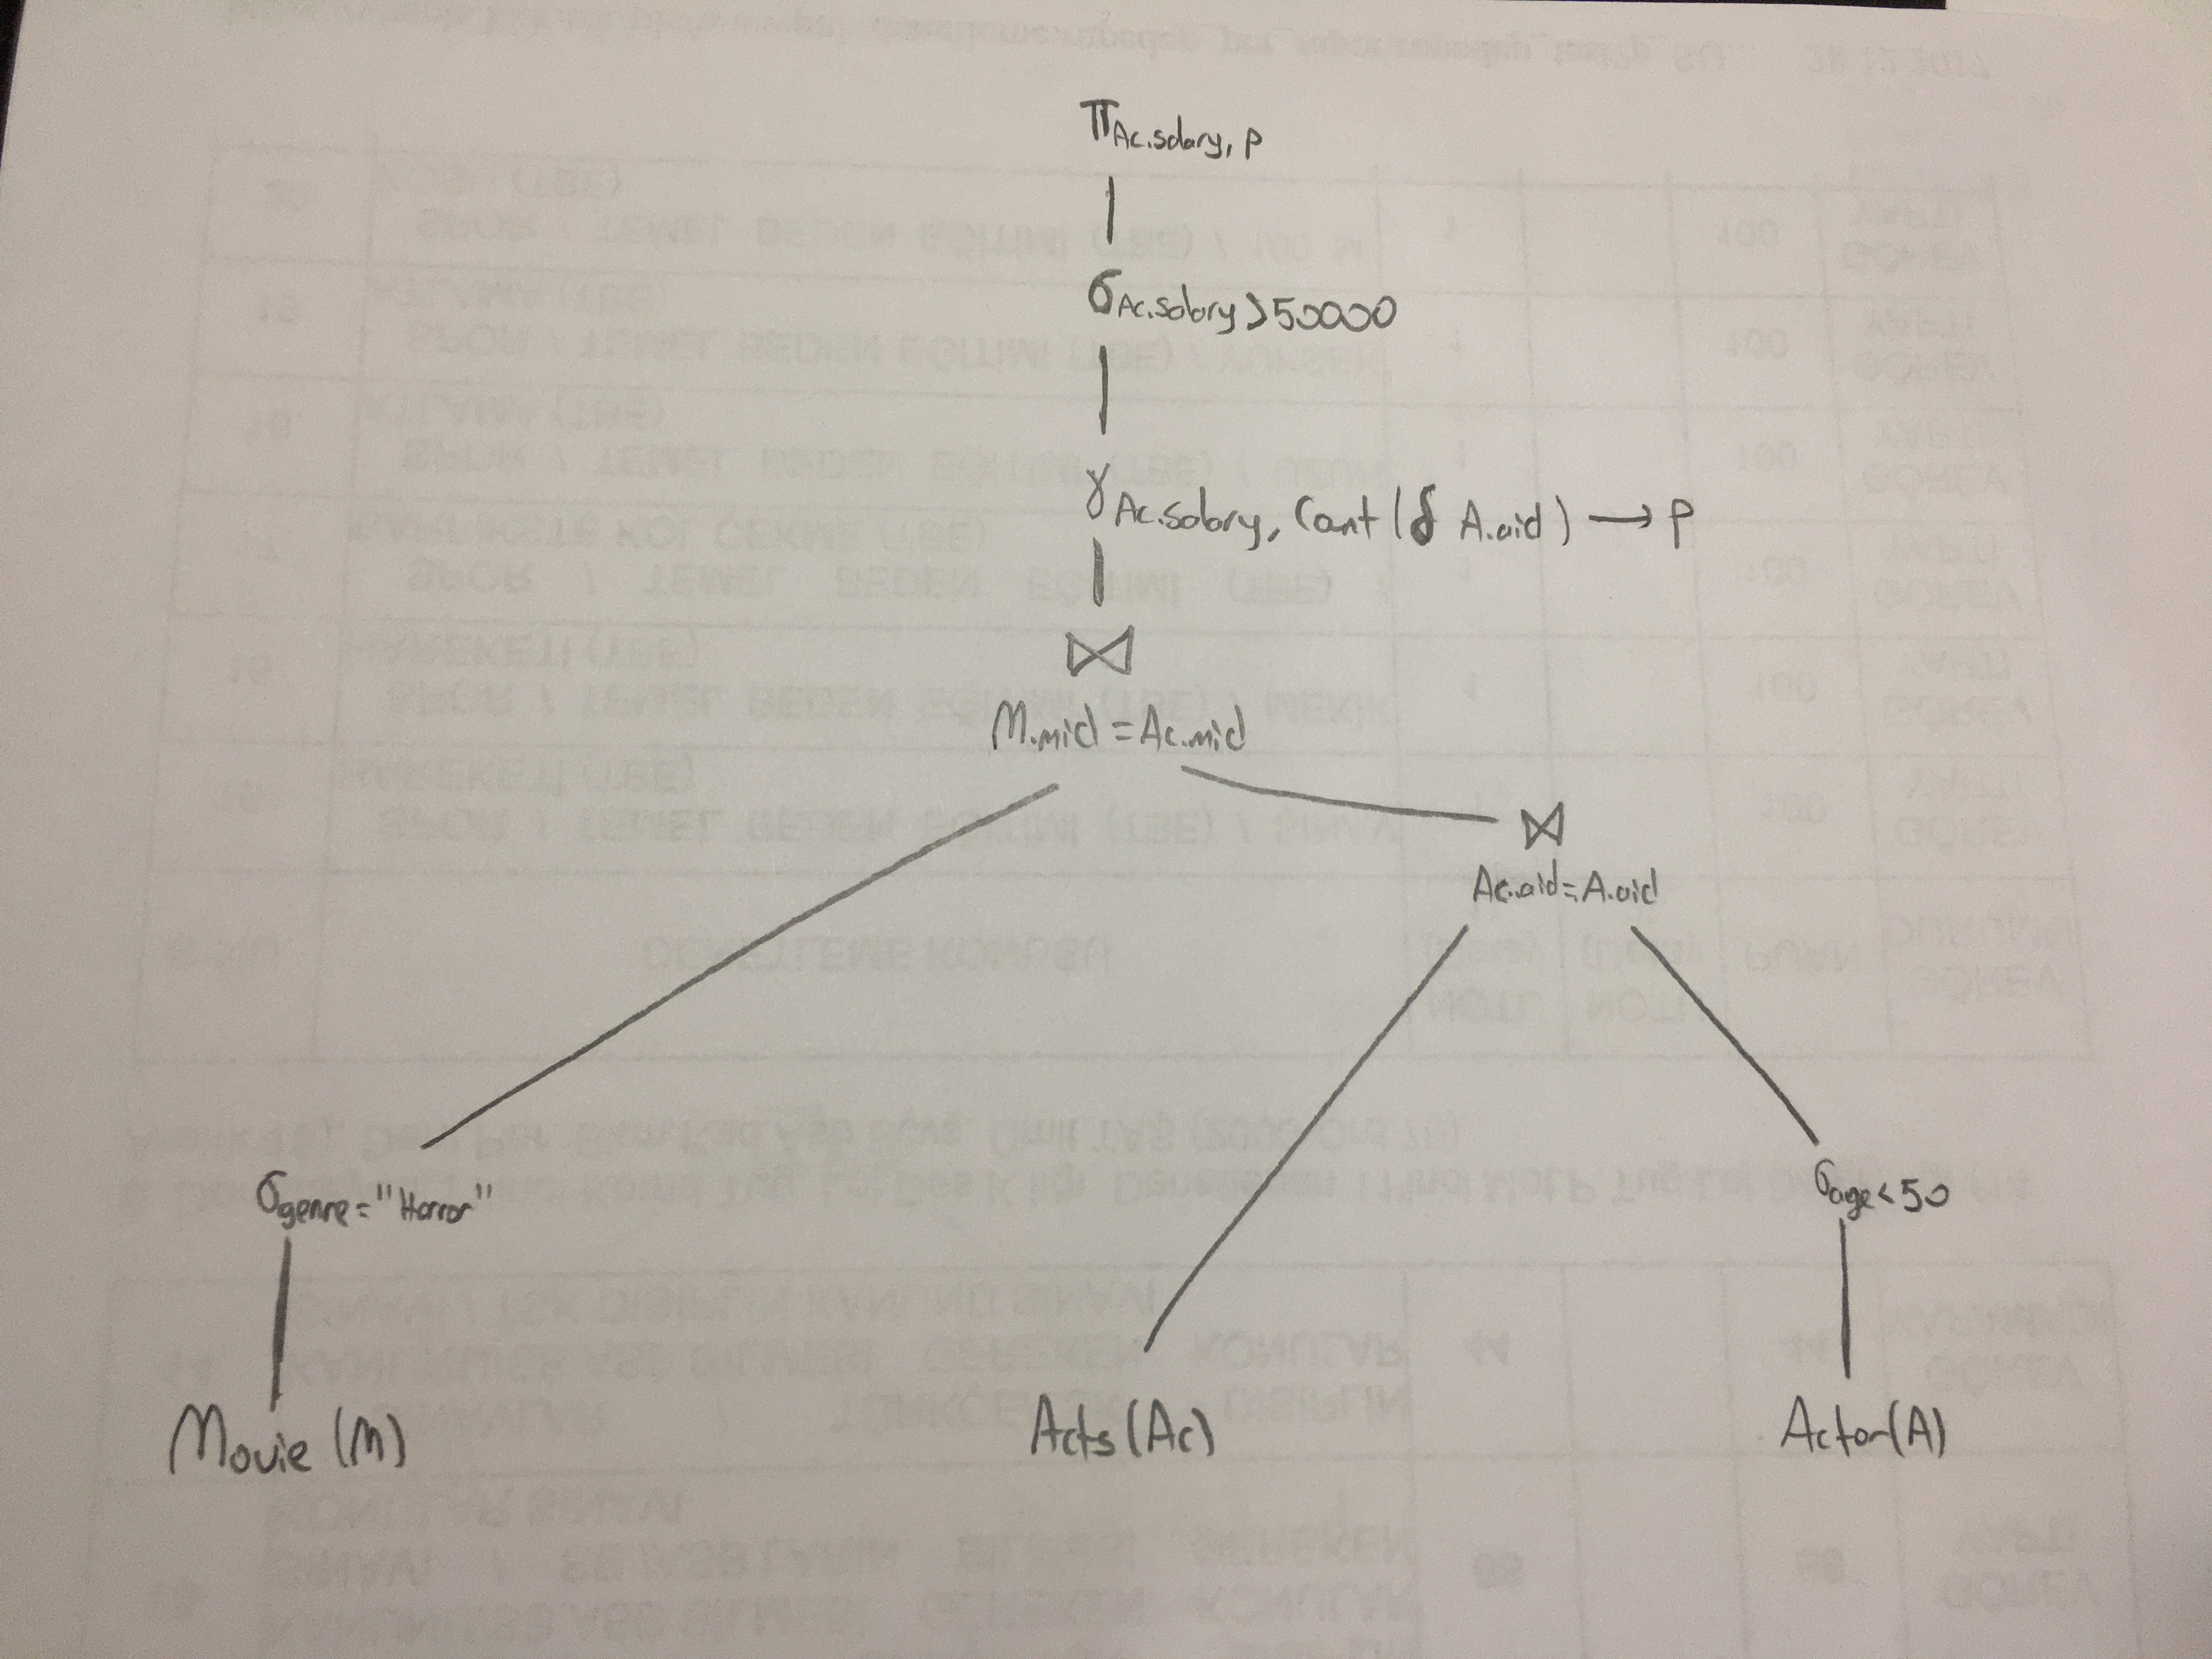
\includegraphics[scale=0.125]{IMG_2456.JPG}
\paragraph{b)} An equivalent logical query plan for this one is: \\
\includegraphics[scale=0.125]{IMG_2458.JPG}
    
\section{Q4}

We are given a join operation on fields of 2 relations and given some information about the relations. We're required to determine the cost of the operations stated in below sections according to the used join algorithm. I am summing up the information given in cost format in below:

\begin{center}
    $T(R) = 20000$ and 10 tuples per page means $B(R) = 2000$ \\
    $T(S) = 5000$ and 10 tuples per page means $B(S) = 500$ \\
    $M = 42$ pages
\end{center}

\paragraph{a)} Cost of joining R and S using a block nested loops join, assuming R is the outer relation can be calculated by $B(R) + B(R)\times B(S)$ which is $2000 + 2000\times 500 = 1002000$ I/Os.

\paragraph{b)} Cost of joining R and S using a block nested loops join, assuming S is the outer relation can be calculated by $B(S) + B(S)\times B(R)$ which is $500 + 500\times 2000 = 1000500$ I/Os.

\paragraph{c)} While joining R and S using a sort-merge join, we're going go through three steps to complete this operation. But first in order to apply this join on these relations we need to have the following condition to be met: $M_1+M_2 \leq M$, ($M_1=B(R)/M$, $M_2=B(S)/M$) checking this condition: $48+12 \leq 60$ which does not hold. Therefore sort-merge join is inapplicable in this situation. However I am going to apply it below by merging $M_1$ and $M_2$ in itself further.

So passing onto description of steps, first we are going to generate initial runs for $R$ by reading first from the disk, then sorting in memory and then writing back to disk. We will go through the same procedure for relation $S$ also. Then finally we are going to merge runs of relations and join them with each other at the same time by reading them again from the disk run-by-run and then joining them on memory and then writing back to disk. Let us show that by the information given to us:

\begin{enumerate}
    \item We have $B(R)=2000$ and an $M=42$ pages. According to this setup we are going to have $M_1=48$ runs. All of these runs will be read from the disk into memory, then they will be sorted in the memory and then written back to disk. At the end we will end up with a relation $R$ divided into 48 sorted (in itself) runs on the disk.
    \item We have $B(S)=500$ and an $M=42$ pages. According to this setup we are going to have $M_2=12$ runs. All of these runs will be read from the disk into memory, then they will be sorted in the memory and then written back to disk. At the end we will end up with a relation $S$ divided into 12 sorted (in itself) runs on the disk.
    \item So now in the merge and join phase, we have 12 sorted runs of $S$ and 48 sorted runs of $R$. Since we have a constraint $M_1+M_2 \leq M$ that does not hold, we need to first pre-merge sorted runs of $R$ and $S$ in themselves into smaller runs. After applying these merges we will have a total number of runs that holds the $M_1+M_2 \leq M$ constraint. Now merge \& join operation will be applied by reading all those runs 1 page at a time (with that we are going to get the pages that corresponds to each other by the magnitude of the values, since they're all sorted) into memory. At each merge \& join operation, output will be written into the output buffer.
\end{enumerate}

The total cost of this operation is given as $3B(R) + 3B(S)$ which is $3\times 2000 + 3\times 500 = 7500$ I/Os.

\paragraph{d)} While joining R and S using a hash join, we're again going go through three steps to complete this operation. But first in order to apply this join on these relations we need to have the following condition to be met: $min(B(R), B(S)) \leq M^2$, checking this condition: $min(2000, 500) \leq 1764$ which holds. So passing onto description of steps, we are first going to hash $R$ into $M-1=41$ buckets and then write all these buckets to disk. Then apply the same exact procedure for $S$. Finally join these two relations by joining every pair of buckets is memory. Let us show that by the information given to us:

\begin{enumerate}
    \item We have $B(R)=2000$ and an $M=42$ pages. So we are going to create $M-1 = 41$ buckets in memory first. Then read the relation $R$ 1 page at a time and hash the values using the given hash function in the relation into these 41 buckets in memory. While this hashing operation by reading 1 page at a time continues, if a bucket fills up then write it corresponding partition in disk. At the end we get a relation $R$ of 2000 pages back on the disk which split into 41 buckets.
    \item We have $B(R)=500$ and an $M=42$ pages. So we are going to create $M-1 = 41$ buckets in memory again. Then read the relation $S$ 1 page at a time and hash the values using the given hash function in the relation into these 41 buckets in memory. While this hashing operation by reading 1 page at a time continues, if a bucket fills up then write it corresponding partition in disk. At the end we get a relation $S$ of 500 pages back on the disk which split into 41 buckets.
    \item We are going to handle join step in 2 phases which are build and probe phase. In build phase we are going to read a partition of $R$ from the disk and create the Hash Table of this partition in memory using a different hash function. Then we are going to scan the matching part of $S$ from the disk and probe fetched values in the hash table we've just created using the partition fetched from relation $R$. In this way we search for matches between two partitions. If we find a match then we write it into the output buffer. 
\end{enumerate}

The total cost of this operation is given as $3B(R) + 3B(S)$ which is $3\times 2000 + 3\times 500 = 7500$ I/Os.

\paragraph{e)} To join two relations using index-nested loop join if $S$ has a:

\begin{enumerate}[i]
    \item Clustered index on the join attribute 'b': Basically iterate over the blocks of relation $R$ and for each block of $R$ fetch corresponding block from relation $S$. Since the structure of the index is clustered on $S$ (consecutive index values have close data values) we can facilitate the fetch operation from relation $S$ by not fetching related tuple(s) tuple-by-tuple instead we can fetch the data block-by-block. As a result we would have a cost of $B(R) + T(R)B(S)/V(S,b)$. Since join attribute is also the primary key for $S$ we can easily deduce that $V(S,b) = T(S)$. Since we are fetching the primary key field from the relation $S$ it will only have 1 I/O cost, i.e. $B(S)/V(S,b)$ part equals to 1. Normally clustered block structure would minimize the cost of this I/O but since we are retrieving only one primary key field we are unable to facilitate the speed of the query here.  \\
    
    So in our case cost is: $2000 + \frac{20000\times 5000}{5000}=22000$ I/Os.
    \item Unclustered index on the join attribute 'b': Basically again iterate over the blocks of relation $R$ and for each tuple of $R$ fetch corresponding tuple from relation $S$. Since the structure of the index is unclustered on $S$ (consecutive index values does not have close data values) we can not facilitate the fetch operation from relation $S$ as we did in clustered case. As a result we would have a cost of $B(R) + T(R)T(S)/V(S,b)$. Since join attribute is also the primary key for $S$ we can again easily deduce that $V(S,b) = T(S)$. \\
    
    So in our case cost is: $2000 + \frac{20000\times 5000}{5000}=22000$ I/Os.
\end{enumerate}

\section{Q5 - Cardinality Estimation}

We're given a table Sales(month, type, price) and a query on this table.

\paragraph{a)} Given these database statistics about the table, a mathematical expression in terms of these statistics' variables, for the estimate the optimizer would use for the cardinality of this query would be:

\begin{center}
    $T(Q) = N \times (m_{10} + m_{11} + m_{12}) \times \frac{t_{swim}}{N}$
\end{center}
Since in the given query we have a conjunction of 2 filters and we're given all the related statistics about the filter attributes. Going over the filters we see that we need histogram values for last 3 month fields and for a certain "swimsuit" value of type field.

\paragraph{b)} The assumptions involved in this estimate are Uniformity \& Independence; namely we've assumed that all values of the attributes uniformly appear with the same probability and in addition, values of different attributes are independent of each other. \\

In the data we're given, these assumptions may reveal as completely incorrect since we do not have any evidence of Uniformity \& Independence in the histograms of "month" and "type" fields. Values of these attributes may not appear uniformly with the same probability or the values may not be independent of each other.

\end{document}
